\documentclass[11pt]{article}
\usepackage[parfill]{parskip}
\usepackage{graphicx}
\usepackage{wrapfig}
\usepackage{subcaption}
\usepackage[top=1in, bottom=1in, left=1in, right=1in]{geometry}
\bibliographystyle{plain}
\usepackage{amsmath}
\usepackage{amsfonts}
\usepackage{hyperref}
%%%%%%%%%%%%%%%%%%%%%%%%%%%%%%%%%%%%%%%%%%%%%%%%%%%%%%%%%%%%%%%
\usepackage{fancyhdr}
\pagestyle{fancy}
%%% Please add the author's last names
\lhead{Galois TA2 AMIDOL}
\rhead{ASKE Milestone 2}
%%% Please use \cfoot{} to remove page numbers
\cfoot{ }
\renewcommand{\headrulewidth}{0pt}
\renewcommand{\footrulewidth}{0pt}
%%%%%%%%%%%%%%%%%%%%%%%%%%%%%%%%%%%%%%%%%%%%%%%%%%%%%%%%%%%%%%&
\usepackage{titlesec}
\titlespacing{\section}{0pt}{\parskip}{-.5\parskip}
\titlespacing{\subsection}{0pt}{\parskip}{- .5\parskip}
\titlespacing{\subsubsection}{0pt}{\parskip}{- .5\parskip}
\newcommand{\closeup}{\setlength{\itemsep}{-4pt}}

\newcommand{\amidol}{\textsc{AMIDOL}}

\def\signed #1{{\leavevmode\unskip\nobreak\hfil\penalty50\hskip2em
  \hbox{}\nobreak\hfil(#1)%
  \parfillskip=0pt \finalhyphendemerits=0 \endgraf}}

\newsavebox\mybox
\newenvironment{aquote}[1]
  {\savebox\mybox{#1}\begin{quote}}
  {\signed{\usebox\mybox}\end{quote}}

\date{\vspace{-5ex}}
% Use this to get rid of the date

\usepackage{authblk}
\author[1]{Eric Davis}
\author[1]{Alec Theriault}
\author[1]{Max Orhai}
\author[1]{Eddy Westbrook}
\author[1]{Ryan Wright}
\affil[1]{Galois, Inc}

%\setcounter{page}{0}



\title{ASKE Milestone 2 for \amidol{}}

\begin{document}
\maketitle
\vspace{10pt}

\section{Introduction}

Complex system analysis currently requires teams of domain experts, data scientists, mathematicians, and software engineers to support the entire life cycle of model-based inference.  The models that result are often bespoke, lack generalizability, are not performable, and make it difficult to synthesize actionable knowledge and policies from their raw outputs.  In this report we describe the current prototype system for \amidol{}: the Agile Metamodel Interface using Domain-specific Ontological Languages, a project that aims to reduce the overhead associated with the model life cycle and enables domain experts and scientists to more easily build, maintain, and reason over models in robust and highly performable ways, and to respond rapidly to emerging crises in an agile and impactful way.  We discuss the current design principles of the \amidol{} prototype, its capabilities, plans for development, and formal aspects of the system.

\amidol{} is designed to support models in a number of scientific, physical, social, and hybrid domains by allowing domain experts to construct meta-models in a novel way, using visual domain specific ontological languages (VDSOLs).  These VDSOLs utilize an underlying intermediate abstract representation to give formal meaning to the intuitive process diagrams scientists and domain experts normally create.  \amidol{}'s abstract representations are executable, allowing \amidol{}'s inference engine to execute prognostic queries on reward models and communicate results to domain experts. \amidol{} binds results to the original ontologies providing more explainability when compared to conventional methods.

\amidol{} addresses the problem of machine-assisted inference with two high-level goals:

\begin{enumerate}
\item improving the ability of domain experts to build and maintain models and
\item improving the explainability and agility of the results of machine-inference.
\end{enumerate}

Our techniques for achieving these goals incorporate abstract functional representations, intermediate languages, and semantic knowledge representation and binding in graph structures into traditional machine learning and model solution techniques.

\section{VDSOL Definition}

\amidol{} is designed to support the definition of ontological languages which describe systems as formal objects.  Objects for a given domain are organized into \emph{toolkits} consisting of \textbf{nouns} and \textbf{verbs}.  Nouns define elements which make up the state space of a system, and verbs define transitions in the state space.  VDSOLs enable domain experts to build models of complex systems which are easier to maintain, validate, and verify, and avoid common pitfalls of monolithic and hand-coded implementations.  To provide visual context for modelers, \amidol{} supports the use of arbitrary scalable vector graphics (SVGs) to represent nouns and verbs, and features a canvas to draw nouns and verbs with labeled arcs connecting them to provide context.

The goal of \amidol{}'s VDSOLs is to enable domain experts to define their models using an interface and visual language similar to the semi-formal diagrams they use today, but with the advantage that \amidol{}s VDSOLs have formal, executable, meaning.  VDSOLs provide a performable, reusable, system for scientists to use when attempting to derive insights relating to the complex systems they represent.

VDSOLs in \amidol{} are constructed using a graphical user interface implemented using asynchronous javascript and XML to build a responsive interface to define models of complex systems, reward models used to explore and understand complex system behavior, and to interact with the results of solvers implemented in the Machine-Assisted Inference Engine.

\subsection{Basic Language Properties}
\paragraph{Nouns}: Nouns in \amidol{} represent portions of the model associated with its state space.  The \amidol{} IR translates noun elements into state variables and constants.  Nouns are represented by custom SVGs, and can be connected to verbs which act upon them.  Users can set the label associated with a noun, which impacts the naming of state variables associated with the noun.

\paragraph{Verbs}: Verbs in \amidol{} represent activities or events which can occur in a model, and which act upon nouns changing the state of the system.  Verbs are associated with a few mandatory and optional properties which impact their translation into the intermediate representation.  All verbs have a mandatory rate which defines the rate at which the associated event occurs.  This rate can be dependent on nouns in the model.  Verbs have an optional enabling condition which can be dependent on nouns in the model.  The enabling condition defines that state variable bounds during which the associated event is enabled, and can be specified as an algebraic expression over state variables associated with nouns in a model.  Verbs also have an optional output function which defines which nouns are impacted when the associated event fires.

\subsection{Composability of Atomic Models}

\subsection{UI/UX Design}

\subsection{JSON Export Language}

\section{Abstract Intermediate Representation}

The Abstract Intermediate Representation (IR) for \amidol{} is meant to be a universal way to specify models, regardless of their domain, and provides a Turing-complete way to specify models performably, while avoiding domain specific considerations.

\subsection{Language Properties}

Formally, the IR is a 5-tuple, $(S, E, L, \Phi, \Lambda, \Delta)$ where:
\begin{itemize}
\item $S$ is a finite set of state variables $\{s_0, s_1, \ldots, s_{n-1}\}$ that take on values in $\mathbb{N}$.
\item $E$ is a finite set of events $\{e_0, e_1, \ldots, e_{m-1}\}$ that may occur in the model.
\item $L: S|E \rightarrow \mathbb{N}$ is the event and state variable labeling function that maps elements of $S and E$ into the original ontology.
\item $\Phi: E \times N_0 \times N_1 \times \ldots \times N_{n-1} \rightarrow \{0, 1\}$ is the event enabling predicate.
\item $\Lambda: E \times N_0 \times N_1 \times \ldots \times N_{n-1} \rightarrow (0, \infty)$ is the transition rate specification.
\item $\Delta: E \times N_0 \times N_1 \times \ldots \times N_{n-1} \rightarrow N_0 \times N_1 \times \ldots \times N_{n-1}$ is the state variable transition function specification.
\end{itemize}

Informally the IR represents models defined in a given VDSOL using an formalism based on Generalized Stochastic Petri-nets with inhibitor arcs (which have the result of making Petri-nets Turing complete).  Instead of inhibtor arcs, we utilize the more intuitive and performable method of allowing events to have input predicates ($Phi$) which can be evaluated to determine if an event is enabled, and output predicates which define the side effects of event firing.

\paragraph{State variables}:

\paragraph{Events}:

\paragraph{Input predicates}:

\paragraph{Output predicates}:

\paragraph{Representation}:

\section{Inference Engine}
\paragraph{ODE Solver}:

\paragraph{Numerical Solution}:

\paragraph{Discrete Event Simulation}:

\section{Reward Variables and Reward Models}

The \amidol{} intermediate representation allows for the specification of reward variables or structures over a given model, and the composition of these structures with a model to produce composed models which can then be solved by the inference engine.  Given a model $M = (S, E, L, \Phi, \Lambda, \Delta)$ we define two basic types of rewards structures, rewards over state variable values (rate rewards), and rewards over events (impulse rewards).

\subsection{Rate Reward Variables}

A rate reward is formally defined as a function $\mathcal{R}: P(S, \mathbb{N}) \rightarrow \mathbb{R}$ where $q \in P(S, \mathbb{N})$ is the reward accumulated when for each $(s,n) \in q$ the marking of the state variable $s$ is $n$.  Informally a rate reward variable $x$ accumulates a defined reward whenever a subset of the state variables take on prescribed values.

\subsection{Impulse Reward Variables}

An impulse reward is formally defined as a function $\mathcal{I}: E \rightarrow \mathbb{R}$ where $e \in E, \mathcal(I)_e$ is the reward for the completion of $e$.  Informally an impulse reward variable $x$ accumulates a defined reward whenever the event $e$ fires.

\subsection{Temporal Characteristics of Reward Variables}

Both rate and impulse reward variables measure the behavior of a model $M$ with respect to time.  As such, a reward variable $\theta$ is declared as either an instant-of-time variable, an interval-of-time variable, a time-averaged interval-of-time variable, or a steady state variable.  An instant of time variable $\Theta_t$ is defined as:

\[ \theta_t = \sum_{\nu \in P(S, \mathbb{N})} \mathcal{R}(\nu) \cdot \mathcal{I}^{\nu}_t + \sum_{e \in E} \mathcal{I}(e) \cdot I_t^e\]

Intuitively a rate reward declared as an instant-of-time variable can be used to measure the value of a state variable precisely at time $t$, and an impulse reward declared as an instant-of-time variable can be used to measure whether a given event fired at precisely time $t$.  While the latter is not a particularly useful measure (as the probability of an event with a firing time drawn from a continuous distribution at time $t$ is $0$) it is defined for closure reasons, and for cases with discrete distributions and discrete time steps.

An interval-of-time variable intuitively accumulates reward over some fixed interval of time $[t, t+1]$.  Given such a variable $\theta_{[t, t+1]}$ we formally define interval-of-time variables as:

\[\theta_{[t,t+1]} = \sum_{\nu \in P(S, \mathbb{N})} \mathcal{R}(\nu) \cdot \mathcal{J}^{\nu}_{[t, t+1]} + \sum_{e \in E} \mathcal{I}(e)N^e_{[t,t+1]}\]

where

\begin{itemize}
\item $J^{\nu}_{[t,t+1]}$ is a random variable which represents the total time the model spent in a marking such that for each $(s, n) \in \nu$, the state variable $s$ has a value of $n$ during the period $[t, t+1]$.
\item $I^e_{t\rightarrow\infty}$ is a random variable which represents the number of times an event $e$ has fired during the period $[t, t+1]$.
\end{itemize}

Time-averaged interval of time variables quantify accumulated reward over some interval of time.  Such a variable $\theta'_{[t,t+1]}$ is defined formally as:

\[\theta'_{[t,t+1]} = \frac{\theta_{[t,t+1]}}{l}\]

\subsection{Translation of Reward Variables to IR}

\subsection{Expressions on Reward Variables}

\section{Design of Experiments and Results Database}
\subsection{Results Database}

\subsection{Prognostic Queries}

\subsection{Model Comparison}

\subsection{Design of Experiments}

\subsection{Conterfactural Exploration, Planning, Crisis Response}

\subsection{Correctness and Uncertainty}

\subsection{Communication of Results}

\section{Domain Models}

We are currently testing \amidol{} using several domain models whose primary domain is epidemiology.  We have selected a range of models to test different scenarios, use cases, and assumptions to aid in the prototype design of \amidol{}.

\subsection{SIS/SIRS}

The SIS/SIRS model is one of the simplest models we have deployed for testing with \amidol{}, with the advantage that the model itself is relatively simple, but utlizes real data, and can be used to answer important epidemiological questions.  The primary objective of the SIS/SIRS model is to identify the \emph{basic reproduction number} associated with an infection, also known as $R_0$, or \emph{r nought}.  $R_0$ was first used in 1952 when studying malaria and is a measure of the potential for an infection to spread through a population.  If $R_0 < 1$, then the infection will die out in the long run.  If $R_0 > 1$, then the infection will spread.  The higher the value of $R_0$, the more difficult it is to control an epidemic.

Given a 100\% effective vaccine, the proportion of the population that needs to be vaccinated is $1 - 1/R_0$, meaning that $R_0$ can be used to plan disease response.  This assumes a homogenous population, and contains many other simplifying assumptions and does not generalize to more complex numbers.  We have several main goals for SIS/SIRS models:

\begin{enumerate}
\item Fitting the models for the data in hindsight to perform goodness of fit estimates.
\item Finding the \emph{retrospective} $R_0$ estimate over the entire epidemic curve.
\item Finding the \emph{real-time} $R_0$ estimate while the epidemic is ongoing.
\end{enumerate}

\paragraph{Data}: For these models we will be working with the WHO/NREVSS (World Health Organization/National Respiratory and Enteric Virus Surveillance System) data sets at the resolution of Department of Human and Health Services designated regions.

\begin{figure}
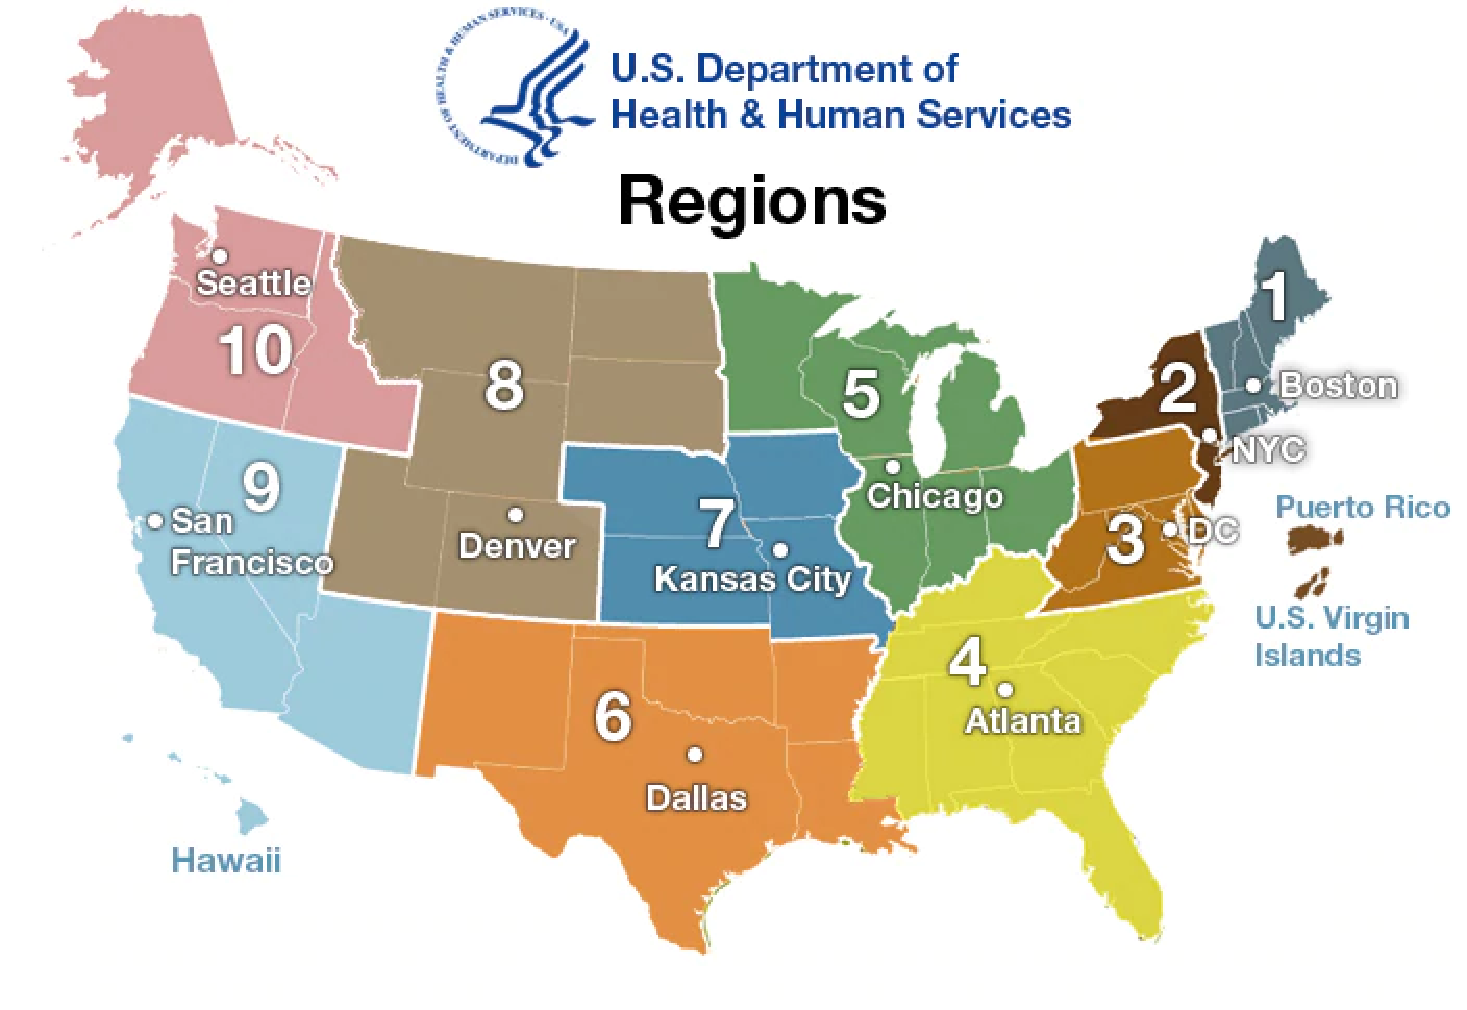
\includegraphics[width=\textwidth]{figs/regionsmap.pdf}
\caption{Department of Human and Health Services designated regions.}
\label{Fig:Regions}
\end{figure}

Using data from a given region, and a given strain, we will estimate R0 for the epidemic curve as shown in Figure \ref{Fig:R0}

\begin{figure}
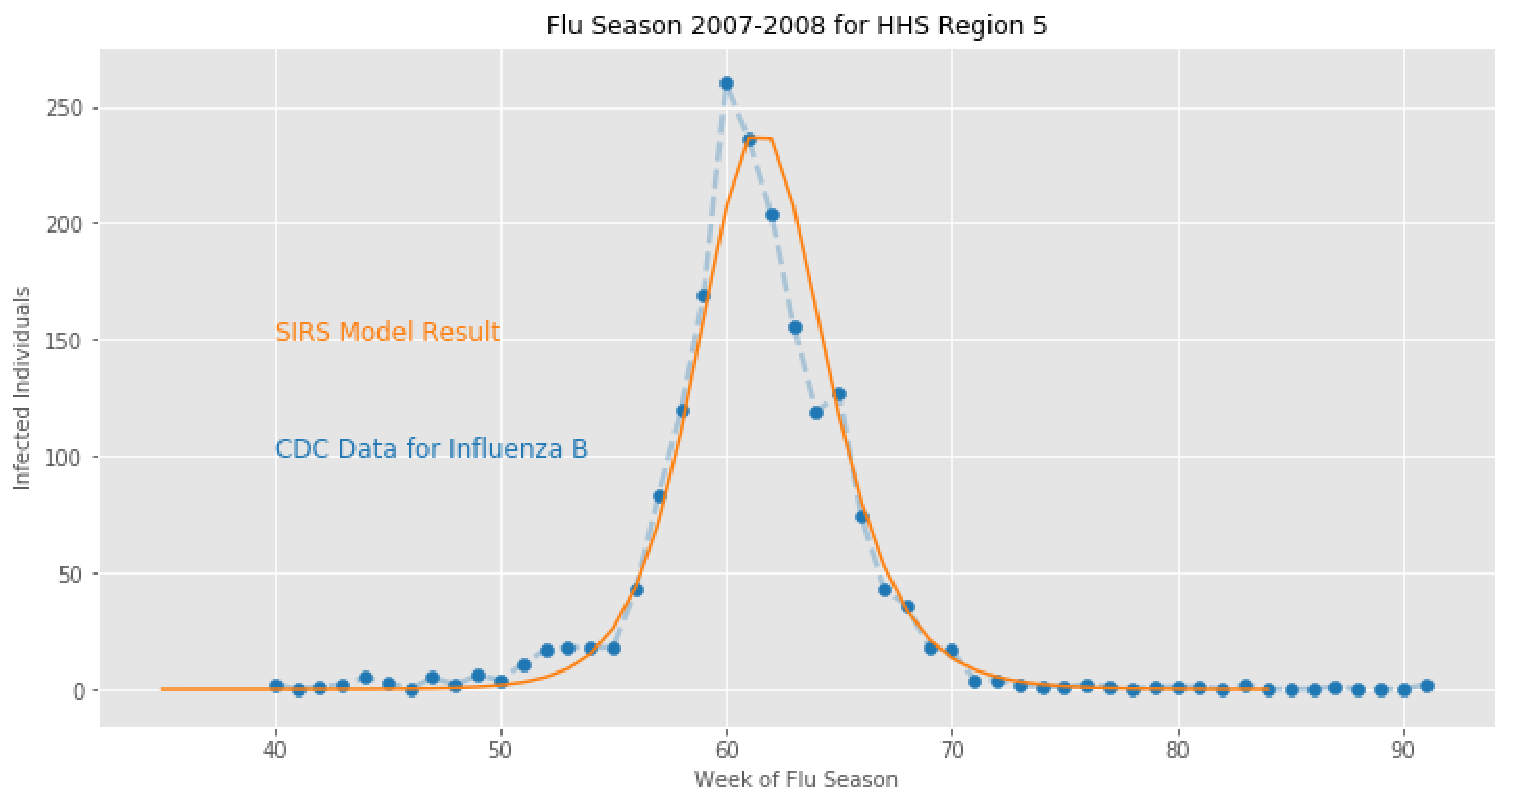
\includegraphics[width=\textwidth]{figs/2007-2008-SIRS.pdf}
\caption{2007 - 2008 Flu Season}
\label{Fig:R0}
\end{figure}

\subsection{Artificial Chemistry}

\subsection{Viral Infection Model}

\begin{figure}
\begin{subfigure}[b]{\textwidth}
\includegraphics[width=\textwidth]{figs/HIV-Tat-figure.pdf}
\caption{Semi-formal diagram of the molecular model of the Tat transactivation circuit.}
\label{Fig:HIV-Tat}
\end{subfigure}
\begin{subfigure}[b]{\textwidth}
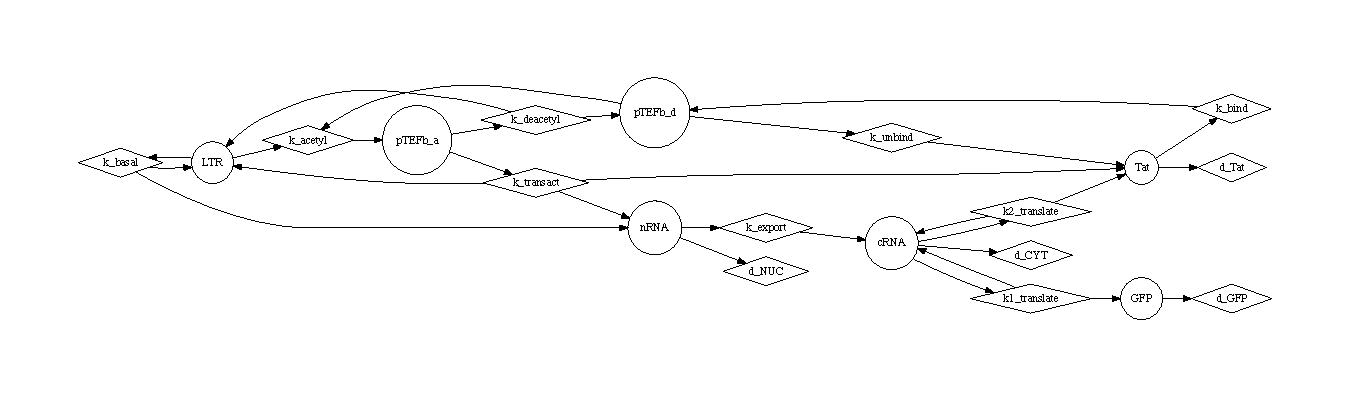
\includegraphics[width=\textwidth]{figs/TatModel.pdf}
\caption{Simple noun (circle) and verb (square) representation of Tat model without ambiguity and aliasing.}
\label{Fig:HIV-Tat-VDSOL}
\end{subfigure}
\end{figure}

Note the use of multiple "Tat" symbols in Figure \ref{Fig:HIV-Tat}. Sometimes scientists draw the same symbol multiple places as an "alias" for the same underlying state variable.

\begin{eqnarray}
LTR \overset{k_{basal}}{\rightarrow} LTR + nRNA\\
nRNA \overset{k_{export}}{\rightarrow} cRNA\\
  cRNA \overset{k1_{translate}}{\rightarrow} GFP + cRNA\\
  cRNA \overset{k2_{translate}}{\rightarrow} Tat + cRNA\\
  Tat \overset{k_{bind}/k_{unbind}}{\leftrightarrow} pTEFb_d\\
  LTR + pTEFb_d \overset{k_{acetyl}/k_{deacetly}}{\leftrightarrow} pTEFb_a\\
  pTEFb_a \overset{k_{transact}}{\leftrightarrow} LTR + nRNA + Tat\\
  GFP \overset{d_{GFP}}{\rightarrow} \emptyset\\
  Tat \overset{d_{Tat}}{\rightarrow} \emptyset\\
  cRNA \overset{d_{CYT}}{\rightarrow} \emptyset\\
  nRNA \overset{d_{NUC}}{\rightarrow} \emptyset
\end{eqnarray}

\subsection{H5N1 Model}

\subsection{H3N2 Model}

\section{User Stories}

\section{Code Repositories and Current Builds}

\begin{figure}
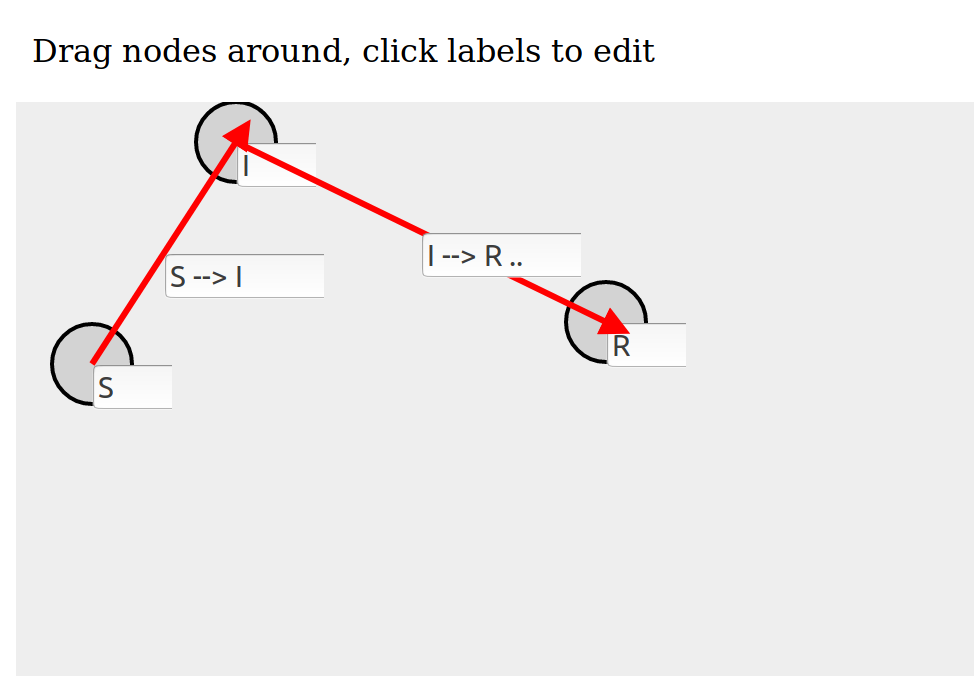
\includegraphics[width=\textwidth]{figs/Editor.png}
\caption{}
\label{Fig:Editor}
\end{figure}

\begin{figure}
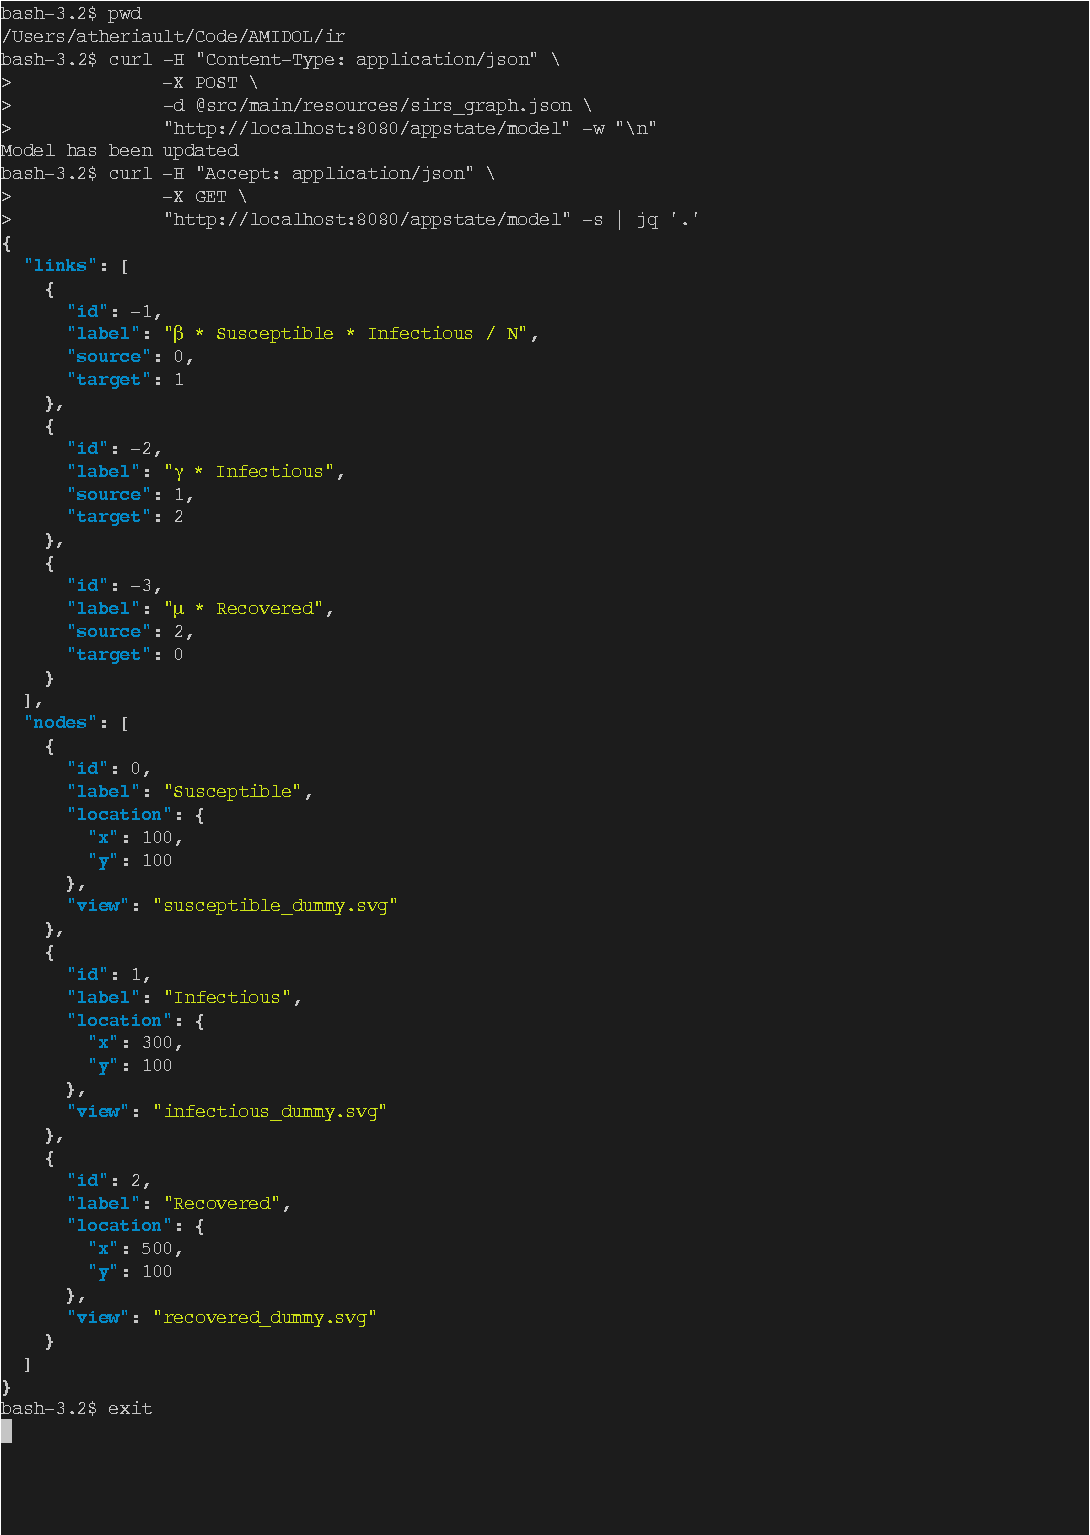
\includegraphics[width=\textwidth]{figs/LoadModel-crop.pdf}
\caption{}
\label{Fig:LoadModel}
\end{figure}

\begin{figure}
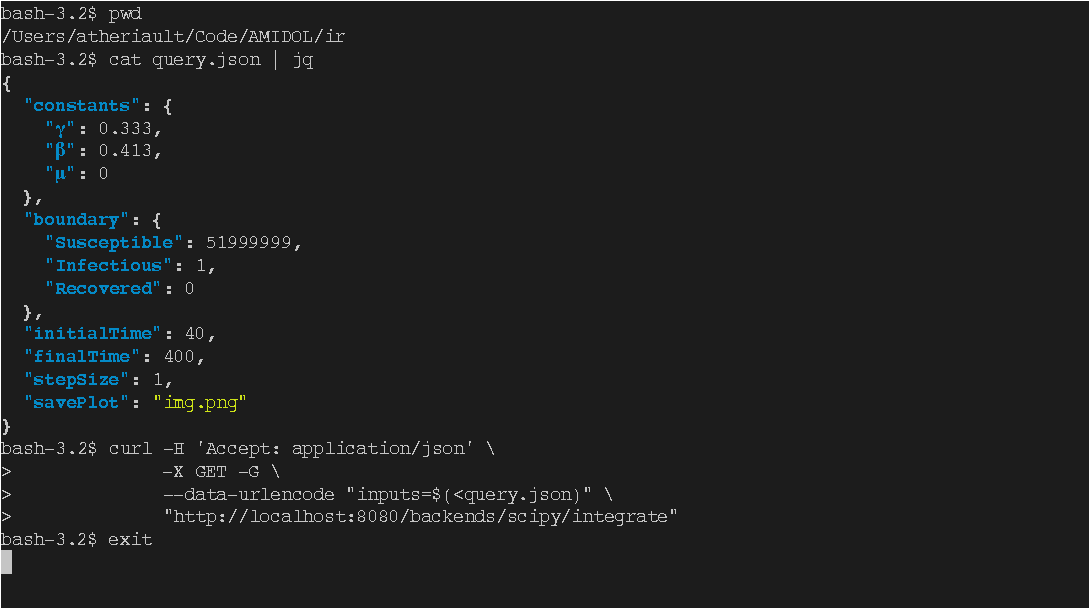
\includegraphics[width=\textwidth]{figs/QueryIntegrateBackend-crop.pdf}
\caption{}
\label{Fig:Query}
\end{figure}

\begin{figure}
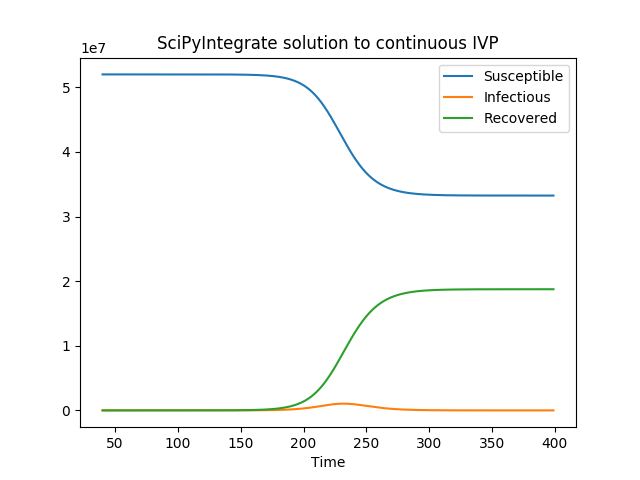
\includegraphics[width=\textwidth]{figs/QueryResult.png}
\caption{}
\label{Fig:QueryResult}
\end{figure}

\section{Roadmap for Future Development}

\bibliography{AMIDOL-MWS}



\end{document}
